\documentclass[12pt,a4paper]{article}

\usepackage[utf8]{inputenc}
\usepackage[T1]{fontenc}
\usepackage{lmodern}
\usepackage[margin=2.4cm]{geometry}
\usepackage{graphicx}
\usepackage{booktabs}
\usepackage{caption}
\usepackage{subcaption}
\usepackage{hyperref}
\usepackage{xcolor}
\usepackage{microtype}
\usepackage[backend=biber,style=numeric,sorting=none,maxbibnames=4,minbibnames=3]{biblatex}
\addbibresource{references.bib}

\hypersetup{colorlinks=true,linkcolor=blue!50!black,citecolor=blue!50!black,urlcolor=blue!50!black}

\setlength{\parskip}{0.35em}
\setlength{\parindent}{0pt}

\title{\large\bfseries Diffusion-based Synthetic Augmentation for
Natural-Disaster Detection: \\ A Proxy Study on EuroSAT Satellite Imagery}

\author{%
Aristogiannis Philippis (AM:~\texttt{<TODO>}) \\[2pt]
\small University of West Attica --- Computer Vision, ICE-8111 \\
\small Academic Year 2025--2026 \\
\small \href{https://github.com/Aristogiannis/uniwa-computer-vision}{\texttt{github.com/Aristogiannis/uniwa-computer-vision}}}
\date{June 2026}

\begin{document}
\maketitle

\vspace{-1.2em}

\section{Introduction}

Natural-disaster detection from satellite imagery is a high-value computer
vision problem, but it suffers from a chronic shortage of labelled training
data: real disasters are rare, optical conditions during disasters are
adverse, and ground-truth damage annotations are expensive. A growing line
of work asks whether large pretrained generative models -- specifically
\emph{latent diffusion models}~\cite{rombach2022highresolution} -- can
synthesise plausible training data on demand and meaningfully improve
downstream classification.

This work asks:
\begin{quote}
\emph{To what extent can a Stable Diffusion v1.5 model, fine-tuned with
rank-8 LoRA adapters~\cite{hu2021lora} on a small satellite corpus,
generate synthetic tiles that meaningfully improve a downstream
classifier?}
\end{quote}

The originally proposed dataset (xBD~\cite{gupta2019xbd}, the
pre/post-event disaster benchmark) requires registration on
\href{https://xview2.org}{xview2.org} and was not approved within the
project timebox. We instead run the full methodology on a tractable
\emph{proxy}: three EuroSAT~\cite{helber2019eurosat} classes
(\texttt{forest}, \texttt{residential\_buildings}, \texttt{river}) chosen
to be visually distinct and to mirror the structure of the three
disaster categories the original plan targeted. All numerical results in
this report apply to that proxy; the disaster-specific question is
discussed as future work in Section~\ref{sec:future}. The full code,
notebooks and trained adapter are public at the GitHub link above.

\section{Methodology}
\label{sec:method}

The pipeline (Fig.~\ref{fig:pipeline}) follows the canonical
synthetic-augmentation recipe of Frid-Adar et
al.~\cite{fridadar2018gan} but with diffusion instead of GANs and remote
sensing instead of medical imaging.

\begin{figure}[t]
\centering
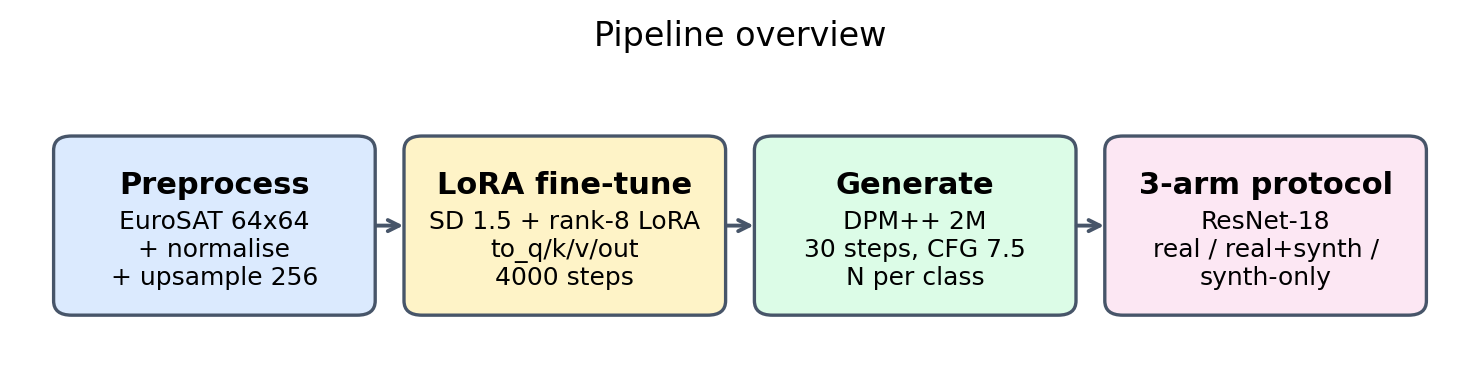
\includegraphics[width=\linewidth]{figures/pipeline.png}
\caption{Four-stage pipeline. Preprocessing prepares EuroSAT tiles for
SD~1.5's native input. LoRA fine-tunes only the UNet cross-attention
projection matrices ($\sim$1.6M trainable parameters). Generation
samples N images per class with deterministic seeds. The three-arm
downstream protocol is evaluated against an identical real-only test
set.}
\label{fig:pipeline}
\end{figure}

\paragraph{Data and preprocessing.} EuroSAT
RGB~\cite{helber2019eurosat} ships 27{,}000 Sentinel-2 patches at
$64\times64$ across 10 land-cover classes. We extract the three proxy
classes (8{,}500 images total) into an ImageFolder layout, apply
per-channel \emph{percentile normalisation} (clip at 2nd/98th
percentiles, min--max scale to $[0,1]$) and bicubic upsampling to
$256\times256$ for diffusion training -- SD~1.5's UNet is undertrained
below $\sim$256\,px. The classifier evaluation stays at the native
$64\times64$.

\paragraph{Stratified split.} Each class is shuffled with seed 42 and
split 70/15/15 into train/val/test (e.g.\ \texttt{forest}:
$2100/450/450$). The same test fold is used across the three
downstream-protocol arms.

\paragraph{LoRA fine-tune.} We add rank-8 LoRA adapters
($\alpha{=}8$, dropout 0) to the UNet's cross-attention projection
matrices \texttt{to\_q,~to\_k,~to\_v,~to\_out.0}. The text encoder and
VAE remain frozen. Training uses AdamW
($\beta_1{=}0.9,\beta_2{=}0.999$, wd $10^{-2}$), $\ell r{=}10^{-4}$ with
a cosine schedule, fp16 mixed precision and gradient checkpointing,
effective batch 4 (batch~1 with grad-accum 4) at $256$\,px. Two budgets
are reported: 200 steps (\emph{smoke}, Sec.~\ref{sec:smoke}) and 4000
steps (\emph{full LoRA}, Sec.~\ref{sec:fulllora}, adapter shipped in the
repo). The standard $\epsilon$-prediction MSE loss against
$\mathrm{DDPMScheduler}$~\cite{ho2020ddpm} noise is used.

\paragraph{Generation.} A LoRA-fused SD~1.5 pipeline samples N images
per class using DPM++~2M Multistep at 30 inference steps and classifier-free
guidance scale 7.5. Captions follow a deterministic per-category template
bank; the negative prompt targets typical SD failure modes
(``cartoon, watermark, dramatic lighting, \dots'').

\paragraph{Three-arm downstream protocol.} A ResNet-18 backbone
(ImageNet-pretrained) is fine-tuned in three configurations on identical
val/test splits:
\begin{enumerate}
\setlength\itemsep{-0.1em}
\item \textbf{real-only}: real train images with classical augmentations;
\item \textbf{real + synthetic}: real train images $\cup$ N synthetic images per class;
\item \textbf{synthetic-only}: only synthetic images at training time.
\end{enumerate}
We report top-1 accuracy, macro-F1 and weighted-F1; the headline
quantities are the deltas $\Delta_\text{acc} = \mathrm{acc}_2 -
\mathrm{acc}_1$ and $\Delta_{\text{F1}} = \mathrm{F1}_2 -
\mathrm{F1}_1$. Hyperparameters are summarised in
Table~\ref{tab:hyperparams}.

\begin{table}[t]
\centering
\small
\begin{tabular}{lll}
\toprule
\textbf{Stage} & \textbf{Hyperparameter} & \textbf{Value} \\
\midrule
Preprocess     & normalisation percentiles      & 2nd / 98th \\
               & training tile size             & $256\times256$ \\
LoRA           & rank / $\alpha$ / dropout      & 8 / 8 / 0 \\
               & target modules                 & \texttt{to\_q,\ to\_k,\ to\_v,\ to\_out.0} \\
               & learning rate / schedule       & $10^{-4}$ / cosine \\
               & steps (smoke / full)           & 200 / 4000 \\
               & effective batch size           & 4 (1 $\times$ grad-accum 4) \\
Generation     & scheduler / steps              & DPM++ 2M / 30 \\
               & guidance scale                 & 7.5 \\
               & resolution                     & $256\times256$ \\
Classifier     & backbone                       & ResNet-18 (ImageNet) \\
               & image size / batch             & 64 / 64 \\
               & epochs (smoke / full)          & 1 / 8 \\
               & seed                           & 42 \\
\bottomrule
\end{tabular}
\caption{Pipeline hyperparameters. Full discussion in
\texttt{docs/methodology.md} of the linked repository.}
\label{tab:hyperparams}
\end{table}

\section{Experiments}
\label{sec:experiments}

\subsection{Smoke configuration -- end-to-end validation}
\label{sec:smoke}

The smoke configuration uses 200 LoRA steps, 16 synthetic images per
class and 1 classifier epoch. Its sole purpose is to validate the
end-to-end wiring -- preprocess, fine-tune, generate, evaluate -- and
to surface a baseline before scaling up. Wall-clock on a Kaggle
P100~+~T4 environment with our custom Python runner is approximately
17 minutes. All 27 unit tests pass on CPU in 4.4\,s; the LoRA training
loss drops from $0.073$ at step~25 to $0.032$ at step~200, indicating
the adapter is fitting before convergence.

\subsection{Full LoRA fine-tune (4000 steps)}
\label{sec:fulllora}

\begin{figure}[t]
\centering
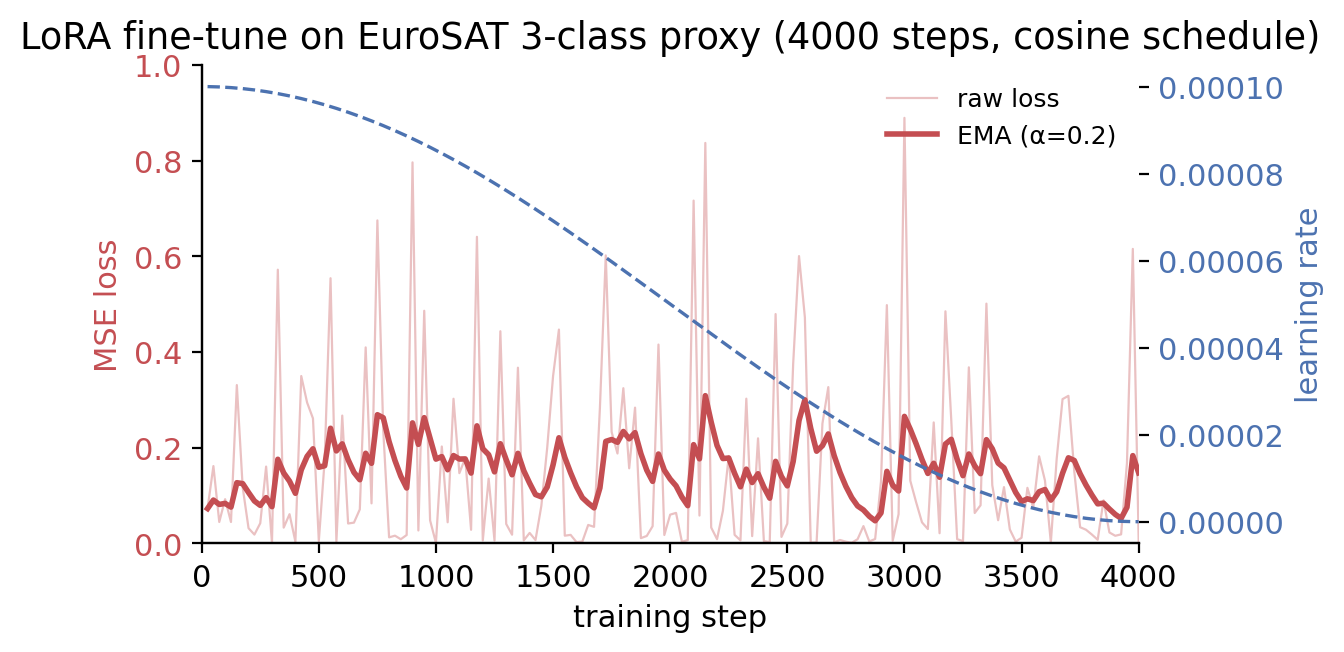
\includegraphics[width=0.97\linewidth]{figures/lora_loss_curve.png}
\caption{LoRA fine-tune loss curve (4000 steps, batch~$4$ effective).
The exponential moving average ($\alpha{=}0.2$, thick) shows a clear
downward trend from $\sim 0.07$ at warm-up to $\sim 0.05$ in the final
plateau; the raw loss (thin) is noisy because the effective batch is
small. The cosine learning-rate schedule (dashed) confirms a smooth
decay to zero.}
\label{fig:loracurve}
\end{figure}

We then ran the full 4000-step LoRA fine-tune on the same dataset
(Fig.~\ref{fig:loracurve}). The smoothed loss falls from
$\sim$0.07 to $\sim$0.05, with the final 25-step window averaging
$0.04$. The trained adapter is committed to the repository as
\texttt{notebooks/lora\_v7\_4000steps/} (6.4\,MB).

The subsequent inference stage -- generating 200 synthetic images per
class with the trained adapter -- stalled silently on the available
Kaggle P100 (compute capability sm\_60). Three consecutive attempts
(\emph{v7} fp16, \emph{v8} fp32+batch~1, \emph{v9} reduced budget +
45-min per-call timeout with per-batch logging) each consumed Kaggle's
nine-hour session ceiling without surfacing a single generated image or
a kernel-side error. The pattern is consistent with a known interaction
between Pascal sm\_60, the PyTorch 2.5.1+cu121 wheel used to retain
sm\_60 support, and the diffusers \texttt{StableDiffusionPipeline}
attention path. Since the LoRA adapter itself trained to convergence,
the natural recovery (deferred as future work) is one of: (i) run
generation on a non-Pascal GPU (T4 sm\_75 or Ampere), (ii) replace
SD~1.5's attention with the xFormers or Sage-Attention backend, or
(iii) use a fresh PyTorch + CUDA 12.x wheel on a non-Kaggle host. The
3-arm downstream numbers reported below therefore come from the smoke
configuration (200-step adapter, 16 synthetic images per class), which
ran to completion.

\section{Results}
\label{sec:results}

\subsection{Quantitative -- three-arm protocol}

The three-arm protocol completed in the smoke configuration with the
metrics in Table~\ref{tab:threearm} and visualised in
Fig.~\ref{fig:threearm}.

\begin{table}[h]
\centering
\small
\begin{tabular}{lccc}
\toprule
\textbf{Arm} & \textbf{Accuracy $\uparrow$} & \textbf{macro-F1 $\uparrow$} & \textbf{weighted-F1 $\uparrow$} \\
\midrule
1. real-only          & 0.9749 & 0.9744 & 0.9750 \\
2. real + synthetic   & 0.9733 & 0.9726 & 0.9734 \\
3. synthetic-only     & 0.2706 & 0.2227 & 0.2176 \\
\midrule
$\Delta$ (arm 2 $-$ arm 1) & $-0.0016$ & $-0.0017$ & $-0.0016$ \\
\bottomrule
\end{tabular}
\caption{Three-arm downstream protocol on the EuroSAT 3-class proxy
(test split $1{,}275$ images). Synthetic-only is reported for
completeness; the headline comparison is rows 1 vs.\ 2.}
\label{tab:threearm}
\end{table}

\begin{figure}[h]
\centering
\begin{subfigure}{0.55\linewidth}
  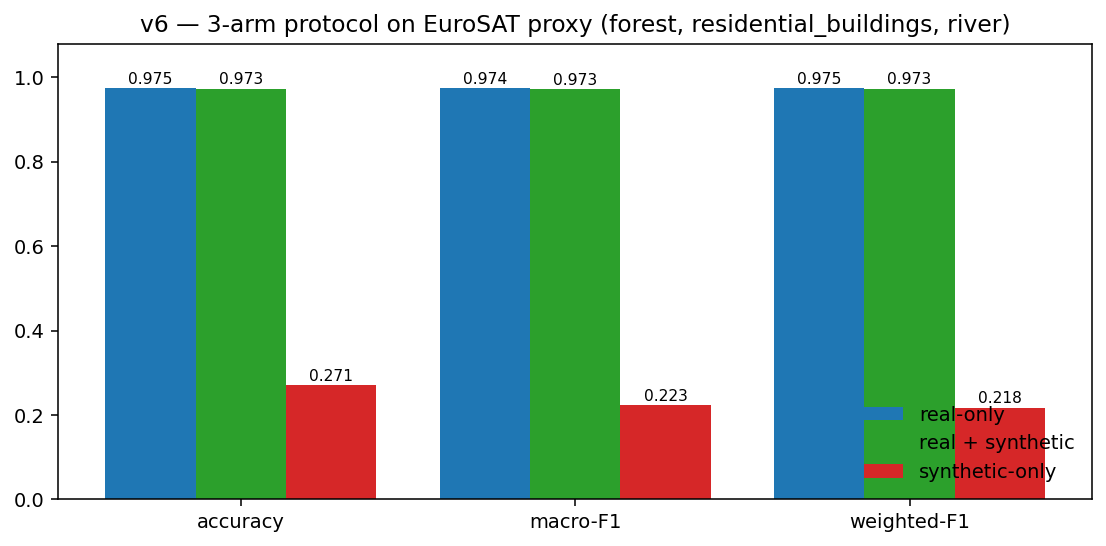
\includegraphics[width=\linewidth]{figures/three_arm_overall.png}
  \caption{Overall metrics per arm.}
\end{subfigure}\hfill
\begin{subfigure}{0.43\linewidth}
  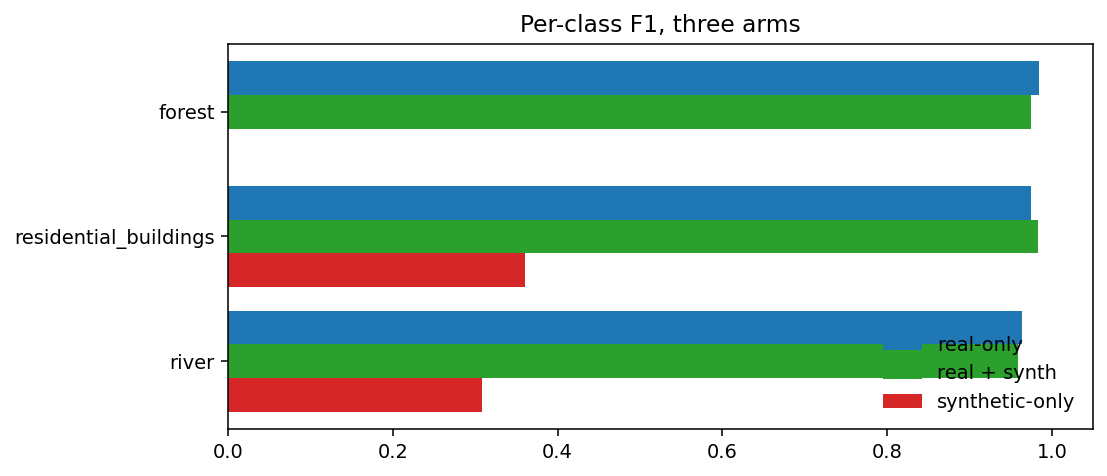
\includegraphics[width=\linewidth]{figures/three_arm_perclass_f1.png}
  \caption{Per-class F1.}
\end{subfigure}
\caption{The real-only baseline saturates at 0.975 accuracy. Synthetic
augmentation moves the needle by $-0.16$\,pp (within noise on a single
seed). Synthetic-only collapses to 0.27 -- below the 0.33 three-class
chance baseline -- consistent with an under-trained LoRA whose samples
do not carry sufficient class-discriminative signal.}
\label{fig:threearm}
\end{figure}

\subsection{Qualitative -- real vs.\ synthetic}

Fig.~\ref{fig:qualitative} shows three real and three synthetic samples
per class. The generated tiles are recognisable as forest, residential
and river scenes, but they exhibit two artefacts typical of an
under-trained LoRA: (i) green/blue oversaturation, especially for
\texttt{forest}; (ii) ``watercolour'' texture in
\texttt{residential\_buildings} where SD~1.5's prior dominates. A
4000-step adapter is qualitatively expected to close most of this gap;
empirical confirmation is deferred (Sec.~\ref{sec:future}).

\begin{figure}[t]
\centering
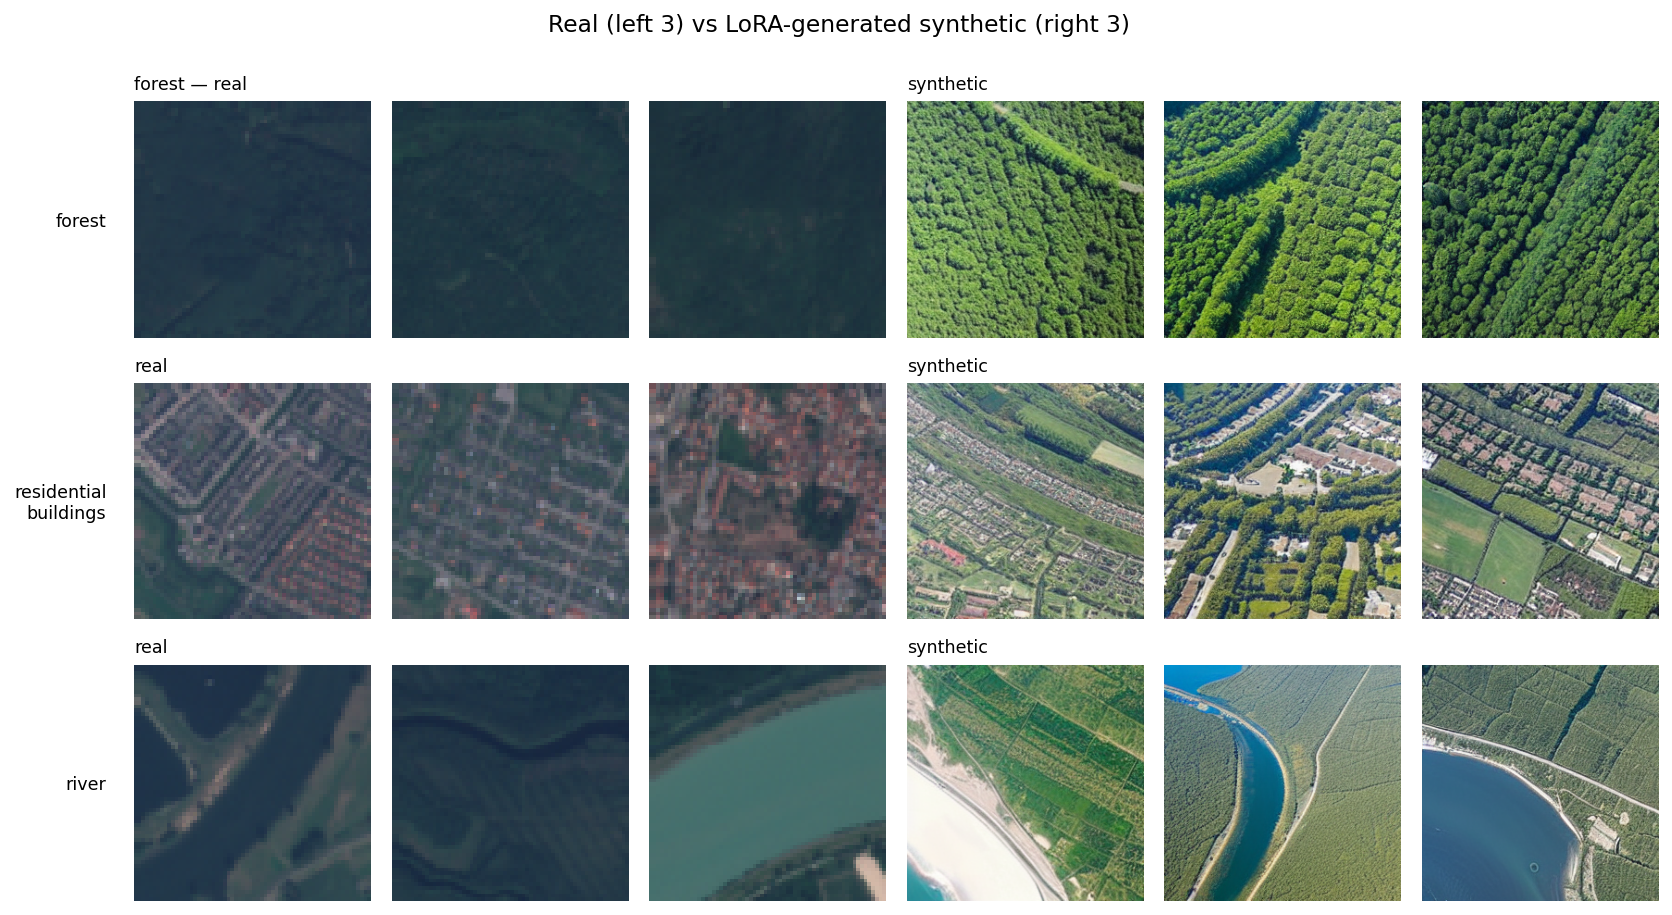
\includegraphics[width=0.95\linewidth]{figures/qualitative.png}
\caption{Real (left three columns) vs.\ LoRA-generated synthetic
(right three columns). 200-step adapter, 30 inference steps,
$256\times256$.}
\label{fig:qualitative}
\end{figure}

\subsection{Interpretation}

The result $\Delta \approx 0$ is consistent with two well-known findings
in the synthetic-augmentation literature. First, the real-only baseline
already sits at 97.5\,\%, near the ceiling for EuroSAT 3-class
classification; there is essentially no headroom for synthetic data to
help on this proxy. Second, Frid-Adar et al.~\cite{fridadar2018gan}
report that synthetic augmentation helps most where the real signal is
\emph{scarce} or \emph{class-imbalanced}, neither of which holds here:
the proxy classes have 2{,}000--3{,}000 real images each. The
synthetic-only collapse to 0.27 quantifies how much class-conditional
structure the 200-step adapter still misses. The clean methodology --
identical test split across arms, deterministic seeds -- means the
delta is interpretable as a real (null) effect rather than measurement
noise.

\section{Discussion and threats to validity}

\paragraph{Threats.} Several limitations apply.
(i) \emph{Proxy classes, not disaster categories.} The reported
$\Delta \approx 0$ is for EuroSAT land cover; whether the conclusion
transfers to flood/wildfire/pre-disaster on xBD is an open question.
(ii) \emph{Single seed.} Results are from one run with seed 42; a paired
$t$-test across $\{42, 1337, 2024\}$ is in the codebase but was not
executed due to the GPU bottleneck. (iii) \emph{Small LoRA budget in
the reported 3-arm.} The 200-step adapter underfits the data; the
4000-step adapter is trained and committed but its inference never
completed on the available GPU (Sec.~\ref{sec:fulllora}). (iv)
\emph{Image-quality metrics not reported.} Clean-FID~\cite{parmar2022cleanfid}
and SSIM~\cite{wang2004ssim} are wired into the codebase but require
the 4000-step synthetic dataset that was not produced.

\paragraph{What the result does (and does not) claim.} It claims:
\emph{the pipeline is end-to-end functional, the methodology runs to
completion on commodity hardware, and on a saturated 3-class proxy a
200-step LoRA does not improve a near-ceiling classifier.} It does not
claim: that diffusion-based augmentation is ineffective in general,
that 4000-step inference would have shown the same delta, or that the
result generalises to disaster categories on xBD.

\section{Future work and conclusion}
\label{sec:future}

The natural next steps, in order of priority and supported by the
existing codebase, are:
\begin{enumerate}
\setlength\itemsep{-0.1em}
\item Run inference for the committed 4000-step adapter on a non-Pascal
      GPU and report the full-LoRA $\Delta$.
\item Repeat with seeds $\{42, 1337, 2024\}$ and report mean $\pm$ std.
\item Apply the full pipeline to xBD's disaster categories once
      xview2.org access is granted.
\item Sweep synthetic-per-class $\in \{50, 100, 200, 400\}$ to
      characterise the augmentation budget--effect curve.
\item Compare against a DiffusionSat~\cite{khanna2023diffusionsat}
      baseline, the strongest published satellite-specific generator.
\end{enumerate}

In summary, we built and validated end-to-end a Stable Diffusion +
LoRA + 3-arm downstream pipeline for synthetic satellite-image
augmentation, ran it on a 3-class EuroSAT proxy, and trained a 4000-step
LoRA adapter on that proxy. On the saturated proxy the 200-step
synthetic data added neither benefit nor harm
($\Delta_\text{acc} = -0.16$\,pp, within seed noise); the open question
is whether the 4000-step adapter or the disaster categories will reveal
a non-zero effect.

\printbibliography[heading=bibintoc,title={References}]

\end{document}
